
% LaTeX Report Template - customizing header and footer
\documentclass[12pt,letterpaper, leqno]{article}
%\documentclass[author]{nrc2}
\usepackage[bottom=1in, top=1in, left=1in, right=1in]{geometry}
\usepackage{amsmath,rotating}
\usepackage[scanall]{psfrag}
\usepackage{setspace}
\usepackage{bm}
\usepackage{lineno}
\usepackage{caption,graphics}
\usepackage{graphicx}
\usepackage{lscape}
\usepackage{natbib}
\usepackage[nottoc]{tocbibind}
\usepackage{indentfirst}
\usepackage{longtable}
\usepackage{sectsty}
\usepackage{color}
\usepackage{fancyhdr}
\usepackage{xspace}
\usepackage{textcomp}
\usepackage{marvosym}

%\usepackage{../MSY}
\bibpunct[, ]{(}{)}{;}{a}{}{,}
\renewcommand\bibname{References}
\renewcommand\figurename{Fig.}
\captionsetup{labelsep=period, singlelinecheck=false}
%\doublespace
\def\little{\fontsize{7pt}{7pt}\selectfont}
\def\Little{\fontsize{10pt}{10pt}\selectfont}
\special{papersize=8.5in,11in}

\newcommand{\diag}{\text{diag}} 
\newcommand{\super}[1]{\ensuremath{^{\text{#1}}}}
\newcommand{\sub}[1]{\ensuremath{_{\text{#1}}}}
\newcommand{\CP}{\ensuremath{\text{CP}}\xspace} 
\newcommand{\SSB}{\ensuremath{\text{SSB}}\xspace} 

\begin{document}
\newcommand{\afrb}{Alaska Fishery Research Bulletin\xspace}
\newcommand{\ajms}{African Journal of Marine Science\xspace}
\newcommand{\amb}{Advances in Marine Biology\xspace}
\newcommand{\bms}{Bulletin of Marine Science\xspace}
\newcommand{\bjssf}{Bulletin of the Japanese Society of Scientific Fisheries\xspace}
\newcommand{\cb}{Conservation Biology\xspace}
\newcommand{\cjfas}{Canadian Journal of Fisheries and Aquatic Sciences\xspace}
\newcommand{\ea}{Ecological Applications\xspace}
\newcommand{\eer}{Evolutionary Ecology Research\xspace}
\newcommand{\elet}{Ecology Letters\xspace}
\newcommand{\emod}{Ecological Modelling\xspace}
\newcommand{\ebf}{Environmental Biology of Fishes\xspace}
\newcommand{\ff}{Fish and Fisheries\xspace}
\newcommand{\fo}{Fisheries Oceanography\xspace}
\newcommand{\fr}{Fisheries Research\xspace}
\newcommand{\fb}{Fishery Bulletin\xspace}
\newcommand{\ijms}{ICES Journal of Marine Science\xspace}
\newcommand{\iccat}{Collective Volume of Scientific Papers ICCAT\xspace}
\newcommand{\jae}{Journal of Animal Ecology\xspace}
\newcommand{\jai}{Journal of Applied Ichthyology\xspace}
\newcommand{\jdc}{Journal Du Conseil International Pour L'exploration De La Mer\xspace}
\newcommand{\jdcp}{Journal Du Conseil Permanent International Pour L'exploration De La Mer\xspace}
\newcommand{\jembe}{Journal of Experimental Marine Biology and Ecology\xspace}
\newcommand{\jfb}{Journal of Fish Biology\xspace}
\newcommand{\jsr}{Journal of Sea Research\xspace}
\newcommand{\jtb}{Journal of Theoretical Biology\xspace}
\newcommand{\jfrbc}{Journal of the Fisheries Research Board of Canada\xspace}
\newcommand{\jnwafs}{Journal of Northwest Atlantic Fisheries Science\xspace}
\newcommand{\mcf}{Marine and Coastal Fisheries: Dynamics, Management, and Ecosystem Science\xspace}
\newcommand{\mb}{Marine Biology\xspace}
\newcommand{\meps}{Marine Ecology Progress Series\xspace}
\newcommand{\mfr}{Marine Fisheries Review\xspace}
\newcommand{\mpb}{Marine Pollution Bulletin\xspace}
\newcommand{\najfm}{North American Journal of Fisheries Management\xspace}
\newcommand{\nzjmfr}{New Zealand Journal of Marine and Freshwater Research\xspace}
\newcommand{\pnas}{Proceedings of the National Academy of Sciences USA\xspace}
\newcommand{\rpvrciemm}{Rapports et Proc\`es-Verbaux des R\'eunions. Conseil Internationale pour l'Exploration de la Mer\xspace}
\newcommand{\rpvrcpiemm}{Rapports et Proc\`es-Verbaux des R\'eunions. Conseil Permanent Internationale pour l'Exploration de la Mer\xspace}
\newcommand{\rfbf}{Reviews in Fish Biology and Fisheries\xspace}
\newcommand{\sajms}{South African Journal of Marine Science\xspace}
\newcommand{\tafs}{Transactions of the American Fisheries Society\xspace}

\newcommand{\anzjs}{Australian \& New Zealand Journal of Statistics\xspace}
\newcommand{\as}{Applied Statistics\xspace}
\newcommand{\csda}{Computational Statistics \& Data Analysis\xspace}
\newcommand{\ees}{Environmental and Ecological Statistics\xspace}
\newcommand{\jas}{Journal of Applied Statistics\xspace}
\newcommand{\jabes}{Journal of Agricultural, Biological, and Environmental Statistics\xspace}
\newcommand{\jasa}{Journal of the American Statistical Association\xspace}
\newcommand{\jrssb}{Journal of the Royal Statistical Society. Series B\xspace}
\newcommand{\sm}{Statistics in Medicine}



\pagestyle{plain}

\begin{titlepage}\center \large

\vspace{144pt}

Relative efficiency of a chain sweep and the rockhopper sweep used for bottom trawl surveys and biomass estimates for flatfish, red hake and goosefish stocks in Northwest Atlantic waters of the United States

\vspace{144pt}

Timothy J. Miller\footnote{Northeast Fisheries Science Center, 166 Water Street, Woods Hole, MA 02543 USA}, 
David E. Richardson, et al.\\

\end{titlepage}

\setcounter{page}{2}
%\linenumbers

\cfoot{\thepage}

\setcounter{page}{2}
\def\fourteenbold{\fontseries{b}\fontsize{14pt}{12pt}\selectfont}
\def\twelvebold{\fontseries{b}\fontsize{12pt}{12pt}\selectfont}
\def\twelveit{\fontshape{it}\fontseries{m}\fontsize{12pt}{12pt}\selectfont}
\sectionfont{\fourteenbold}
\subsectionfont{\twelvebold}
\subsectionfont{\twelvebold}
\subsubsectionfont{\twelveit}

\section*{Abstract}

Using a general hierarchical model we estimated relative efficiency of chain sweep to the rockhopper sweep used by the NEFSC bottom trawl survey for  from studies carried out between 2015 and 2017 aboard the F/V Karen Elizabeth twin-trawl vessel. Aside from the sweeps, the rest of the trawl gear is the same.  We compared a set of models with different assumptions about variation of relative efficiency between paired gear tows, size and diel effects on the relative efficiency, and extra-binomial variation of observations within paired gear tows.  %The best model includes size effects on and variation in relative catch efficiency between each paired tows. Diel effects provided improved model performance. We used the best performing model to make annual chain sweep-based swept area biomass and abundance-at-length estimates. We estimated uncertainty in all results using bootstrap procedures for each data component.

\pagebreak

\section*{Introduction}

Paired-gear studies have long been used to estimate the efficiency of one fishing gear relative to another \citep[e.g.,][]{gulland64,bourne65}.  These types of studies are critical for informing abundance time series from fishery independent surveys when there are changes in the vessel and(or) gears over time due to gear failures or improved technology. 

In conducting paired-gear studies it is ideal to have the two gears deployed as close together spatailly and temporally as possible to reduce variation between the gears in densities of the species being captured. One fishing method that approaches this ideal is the twin-trawl rigging where two trawls can be fished simultaneously \citep{ices96}. The basic methods we used here are the same as those used by \citet{miller13} to estimate size effects on relative catch efficiency of the Henry B. Bigelow to the Albatrosss IV and to make similar estimates for groundfish, TRAC stocks and summer flounder \citet{milleretal17a,milleretal17b}.   

\section*{Methods}

\subsection*{Data collection}

Data were collected during three field experiments carried out in 2015, 2016, and 2017, respectively, aboard the F/V Karen Elizabeth, a 78ft stern trawler capable of towing two trawls simultaneously side by side. However, red hake were only observed during the 2017 field experiments. One side of the twin-trawl rig towed a NEFSC standard 400 x 12 cm survey bottom trawl rigged with the NEFSC standard rockhopper sweep \citep[]{politisetal14} (Figure 1). The other side of the twin-trawl rig towed a version the NEFSC 400 x 12cm survey bottom trawl modified to maximize the capture of flatfish. The trawl was modified by reducing the headline floatation from 66 to 32, 20cm, spherical floats, reducing the port and starboard top wing-end extensions by 50cm each and utilizing a chain sweep. The chain sweep was constructed of 1.6cm (5/8in) trawl chain covered by 12.7cm diameter x 1cm thick rubber discs on every other chain link (Figure 2). Two rows of 1.3cm (1/2in) tickler chains were attached to the 1.6cm trawl chain by 1.3cm shackles (Figure 2). To ensure equivalent net geometry of each gear, 32m restrictor ropes, made of 1.4cm (9/16in) buoyant, Polytron rope, were attached between each of the trawl doors and the center clump. 3.4m2 Thyboron Type 4 trawl doors were used to provide enough spreading force to ensure the restrictor ropes remained taut throughout each tow. Each trawl used the NEFSC standard 36.6m bridles. All tows followed the NEFSC standard survey towing protocols of 20 minutes at 3.0 knots. 103 (61 day, 42 night) paired tows were conducted in waters off of southern New England (Figure \ref{2017_tow_locations}).  Paired tows were denoted as ``day'' and ``night''  by whether the sun was above or below the horizon at the time of the tow. 

Red hake were caught in 73 paired tows (40 day, 33 night). Overall 12,585  red hake were measured for length. The subsampling fractions implied an estimated 47,275 red hake were captured across all paired tows. 8587 and 3998 length measurements were made for the chainsweep and rockhopper gears, respectively.  During the day, 4908 and 1706 red hake were measured in catches by the respective gears whereas during the night 3679 and 2292 were measured in catches by the respective gears.

\subsection*{Paired-tow analyses}

We use the hierarchical modeling approach from \citet{miller13} to estimate the relative efficiency of chain sweep to the rockhopper sweep used by the NEFSC bottom trawl survey for six species from three studies carried out aboard a twin trawl vessel. Aside from the sweeps the rest of the trawl gear is the same.  As in \citet{miller13}, we compared a set of models with different assumptions about variation of relative efficiency between paired gear tows, size effects on the relative efficiency, and extra-binomial variation of observations within paired gear tows. We began with the same 13 models considered by \citet{miller13}, and then also included diel effects on reletive catch efficiency and intereactions with size effects with the best performing model of the original 13 models. Table \ref{models_table} provides a descriptions of the fitted models and pseudo-formulas comparable to those used for fitting models in R and the mgcv package \citep{R19,wood06}. The analyses are analogous to those by \citet{milleretal17a,milleretal17b,milleretal18}, but we have generalized the model fitting software to fit mulitiple smooth effects on relative catch efficiency so that models do not have to be fit separately to observations occurring during the day and night. Therefore when diel effects are considered many parameters can be allowed to be common to the day and night observations. 

\subsection*{Length-weight analysis}

We fit length-weight relationships to the length and weight observations for each survey each year. We assumed weight observation $j$ from survey $i$, was log-normal distributed,
\begin{equation}\label{wal}
 \log W_{ij} \sim \text{N}\left(\log \alpha_i + \beta_i \log L_{ij} - \frac{\sigma_i^2}{2}, \sigma_i^2\right)
\end{equation}
We used a bias correction to ensure the expected weigth $E(W_{ij})= \alpha_i L_{ij}^{\beta_i}$. We estimaed parameters by maximizing the model likelihood programmed in TMB \citep{kristensenetal16} and R \citep{R19}. Like the relative catch efficiency, bootstrap predictions of weight at length were made by sampling with replacement the length-weight observations within each annual survey and refitting the length-weight relationship to each of the bootstrap datasets.


\subsection*{Biomass estimation}

We estimated biomass for each annual survey in terms of chainsweep efficiency by scaling the survey tow observations by the relative efficiency of the chainsweep and rockhopper sweep gears. First the tow-specific catches at length are rescaled,
\begin{equation}\label{nal}
\widetilde N_{hi}\left(L\right) = N_{hi}\left(L\right)\widehat \rho_i\left(L\right)
\end{equation}
where $N_{hi}(L)$ is the number at length $L$ in tow $i$ from stratum $h$ and $\widehat \rho_i\left(L\right)$ is the relative efficiency of the chain sweep to rockhopper sweep at length $L$ estimated from the twin trawl observations, that may depend on the diel characteristic of tow $i$ if that factor is in the best model fitted to the twin-trawl observations. Note that we have omitted any subscripts denoting the year or survey. 

The stratified abundance estimate is then calculated using the design-based estimator, 
\begin{equation}\label{Nal_estimate}
 \widehat N(L) = \sum^H_{h=1} \frac{A_h}{An_h}\sum^{n_h}_{i=1} \widetilde N_{hi}(L)
\end{equation}
where $A_h$ is the area of stratum $h$, $A=\sum^H_{h=1} A_h$, and $n_h$ is the number of tows that were made in stratum h. The corresponding biomass estimate is then
\begin{equation}\label{biomass_estimate}
 \widehat B = \sum^{n_L}_{l=1} \widehat N(L = l) \widehat w(L=l)
\end{equation}
where $\widehat w(L=l)$ is the estimated weight at length from fitting length-weight observations described above. Length is typically measured to the nearest cm so $n_L$ indicates the number of 1 cm length categories that were observed during the survey. 

To estimate uncertainty in biomass, we used bootstrap results for the relative catch efficiency and weight at length estimates along with bootstrap samples of the survey data.  Bootstrap data sets for each of the annual surveys respected the stratified random designs by resampling with replacement within each stratum \citep{smith97}. For each of the 1000 combined bootstraps, survey observations for bootstrap $b$ were scaled with the corresponding bootstrap estimates of relative cookie sweep to rockhopper sweep efficiency and predicted weight at length, using Eqs. \ref{Nal_estimate} and \ref{biomass_estimate}.

\section*{Results}

As measured by AIC, the best performing model before considering day/night effects was the conditional beta-binomial model BB$_6$ (Table \ref{models_table}). The best beta-binomial model had an AIC more than 13 units lower than the best binomial model. Allowing variation in smooth size-effects on relative catch efficiency among paired-tows and extra-binomial variation withing paired-tows  (overdispersion via the beta-binomial assumption) provided primary improvements in model performance. Including diel effects on relative efficiency for the twin-trawl observations improved performance of the beta-binomial model. Initially separate smooth size effects for day and night tows were considered for the beta-binomial model (BB$_8$), but the correlation of non-smoother related random effects across stations was not estimable. Those random effects were therefore assumed uncorrelated (BB$_9$). Allowing different smooth size effects of relative efficiency for day and night observations was considerd (BB$_{10}$), but it did not improve model performance. The relative efficiency of the chain sweep gear to the rockhopper sweep gear generally declines with increased size whether the tow occurred during day or night, but the increase in efficiency of the chainsweep was generally greater for tows occuring during the day (Figure \ref{combined_rhos}). 

Stock-specific trends in annual biomass estimates from 2009 to 2019 for the NEFSC spring and fall survey were generally the same. For northern red hake both the spring and fall biomass estimates increased in 2014 and have remained higher than previous years (Figure \ref{north_red_hake_biomass} and Table \ref{biomass_table}). The scale of the biomass estimates is also similar for the spring and fall surveys. For southern red hake, The spring biomass generally declined until 2017 and then has increaed for the last two years whereas the fall biomass has remained relatively stable (Figure \ref{south_red_hake_biomass} and Table \ref{biomass_table}). 

The efficiency of the rockhopper gear relative to the chainsweep in terms of biomass changes from year to year due primarily to corresponding changes in the estimated numbers at length (Table \ref{biomass_efficiencies}). Annual biomass relative efficiency for northern red hake varied between 0.19 and 0.25 in the spring and 0.21 and 0.33 in the fall. Vaues range between 0.15 and 0.26 for the spring and 0.19 and 0.39 in the fall for southern red hake. 

Because the length-weight relationship which is used with the numbers at length to estimate biomass is estimated by survey and year there is a possiblity that poor sampling in a given year could adversely affect the biomass estimates.  We therefore calculated the ratios of the annual uncalibrated biomass estimates using just the aggregate catch data to the biomass estimates made using the numbers at length and estimated weight at length (i.e., Eqs. \ref{Nal_estimate} and \ref{biomass_estimate} without the relative efficiency at size). These ratios should be approximately 1. The ratios for all years and seasons for both northern and southern red hake varied from 0.96 to 1.04 (Table \ref{biomass_ratios}).


\bibliography{chainsweep_refs}
\bibliographystyle{/home/tmiller2/work/bibliographies/cjfas2}

\clearpage

\begin{figure}
\caption{Diagram of the standard Northeast Fisheries Science Center rockhopper sweep center and wing sections.}\label{rockhopper_schematic}
\begin{center}
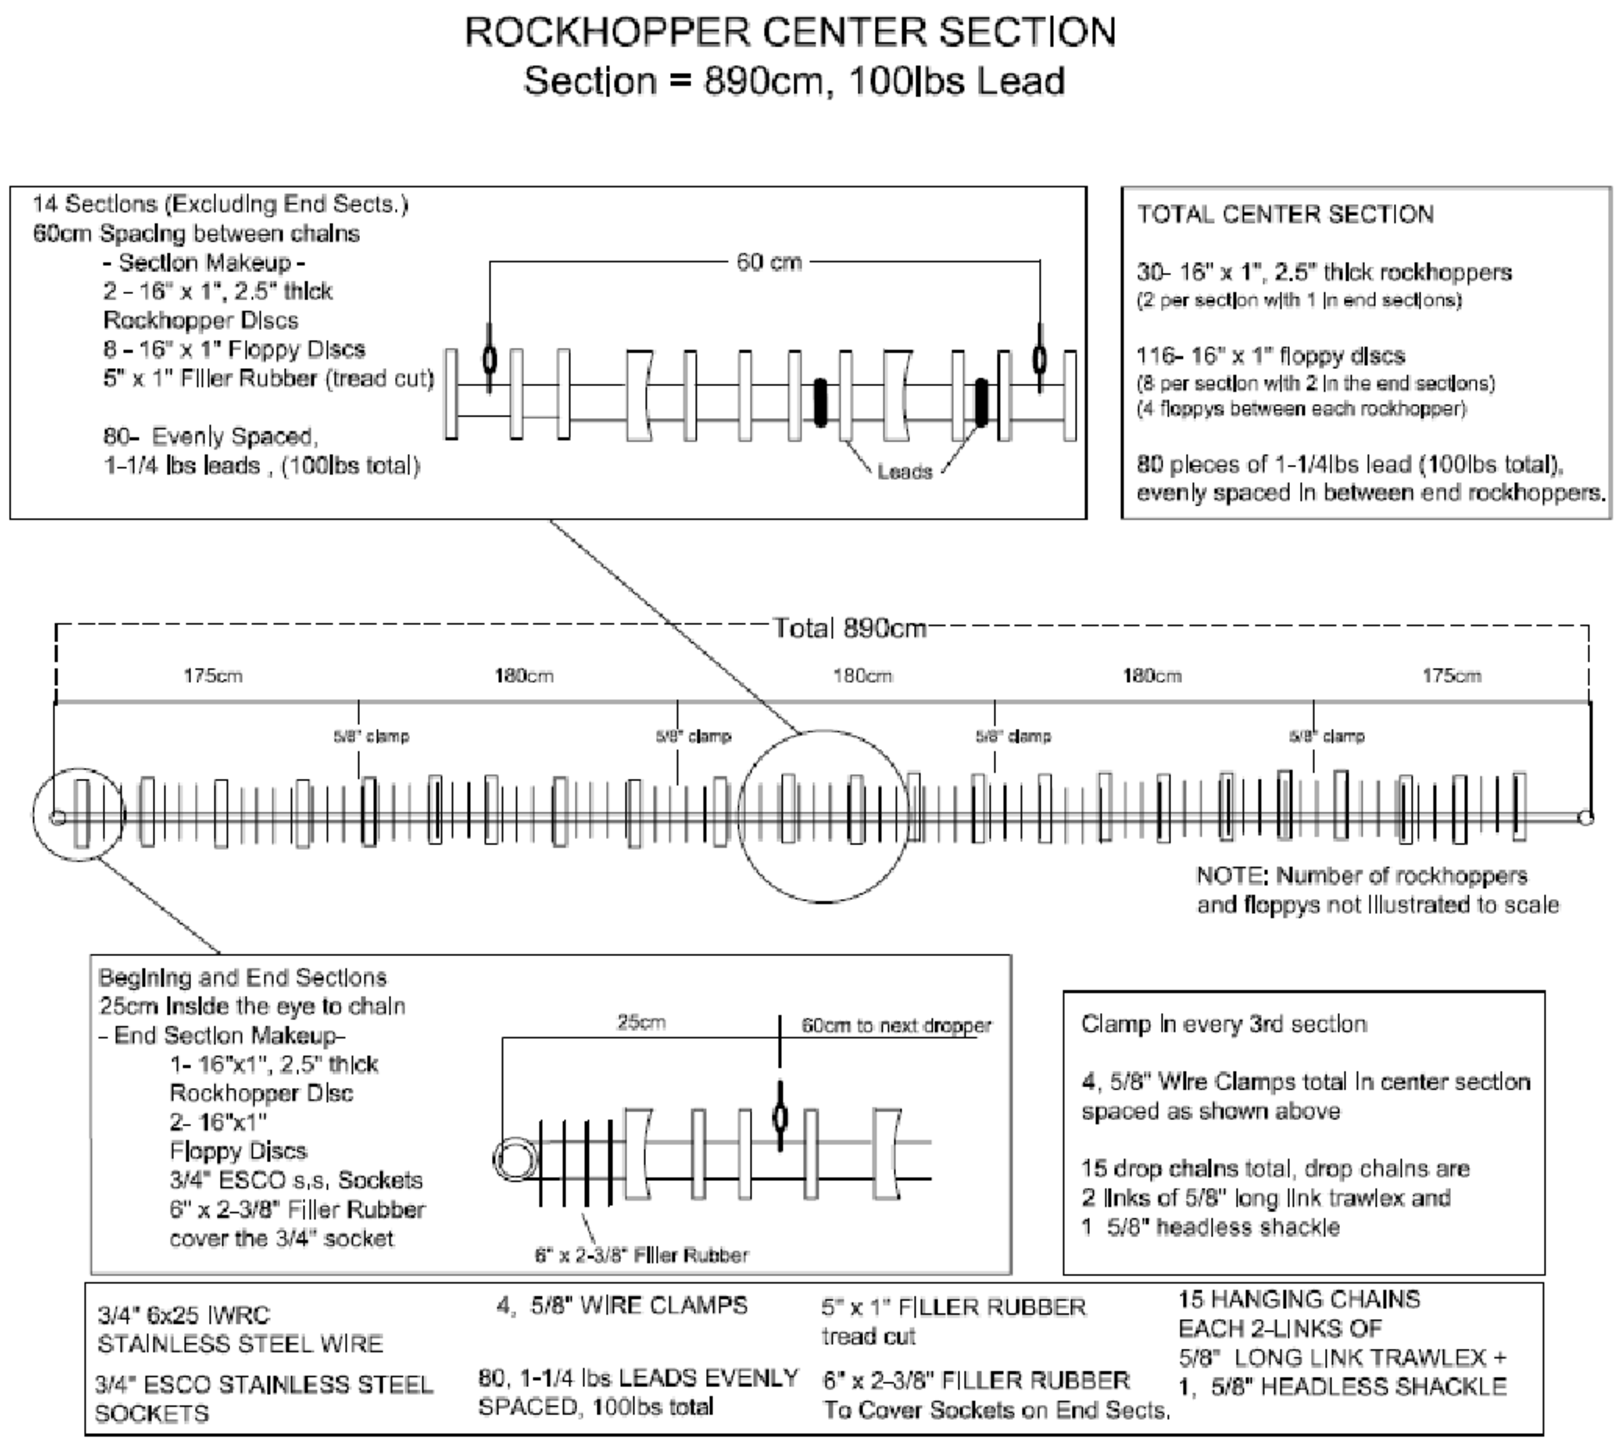
\includegraphics[width = 0.7\textwidth]{rockhopper_schematic_1.pdf}
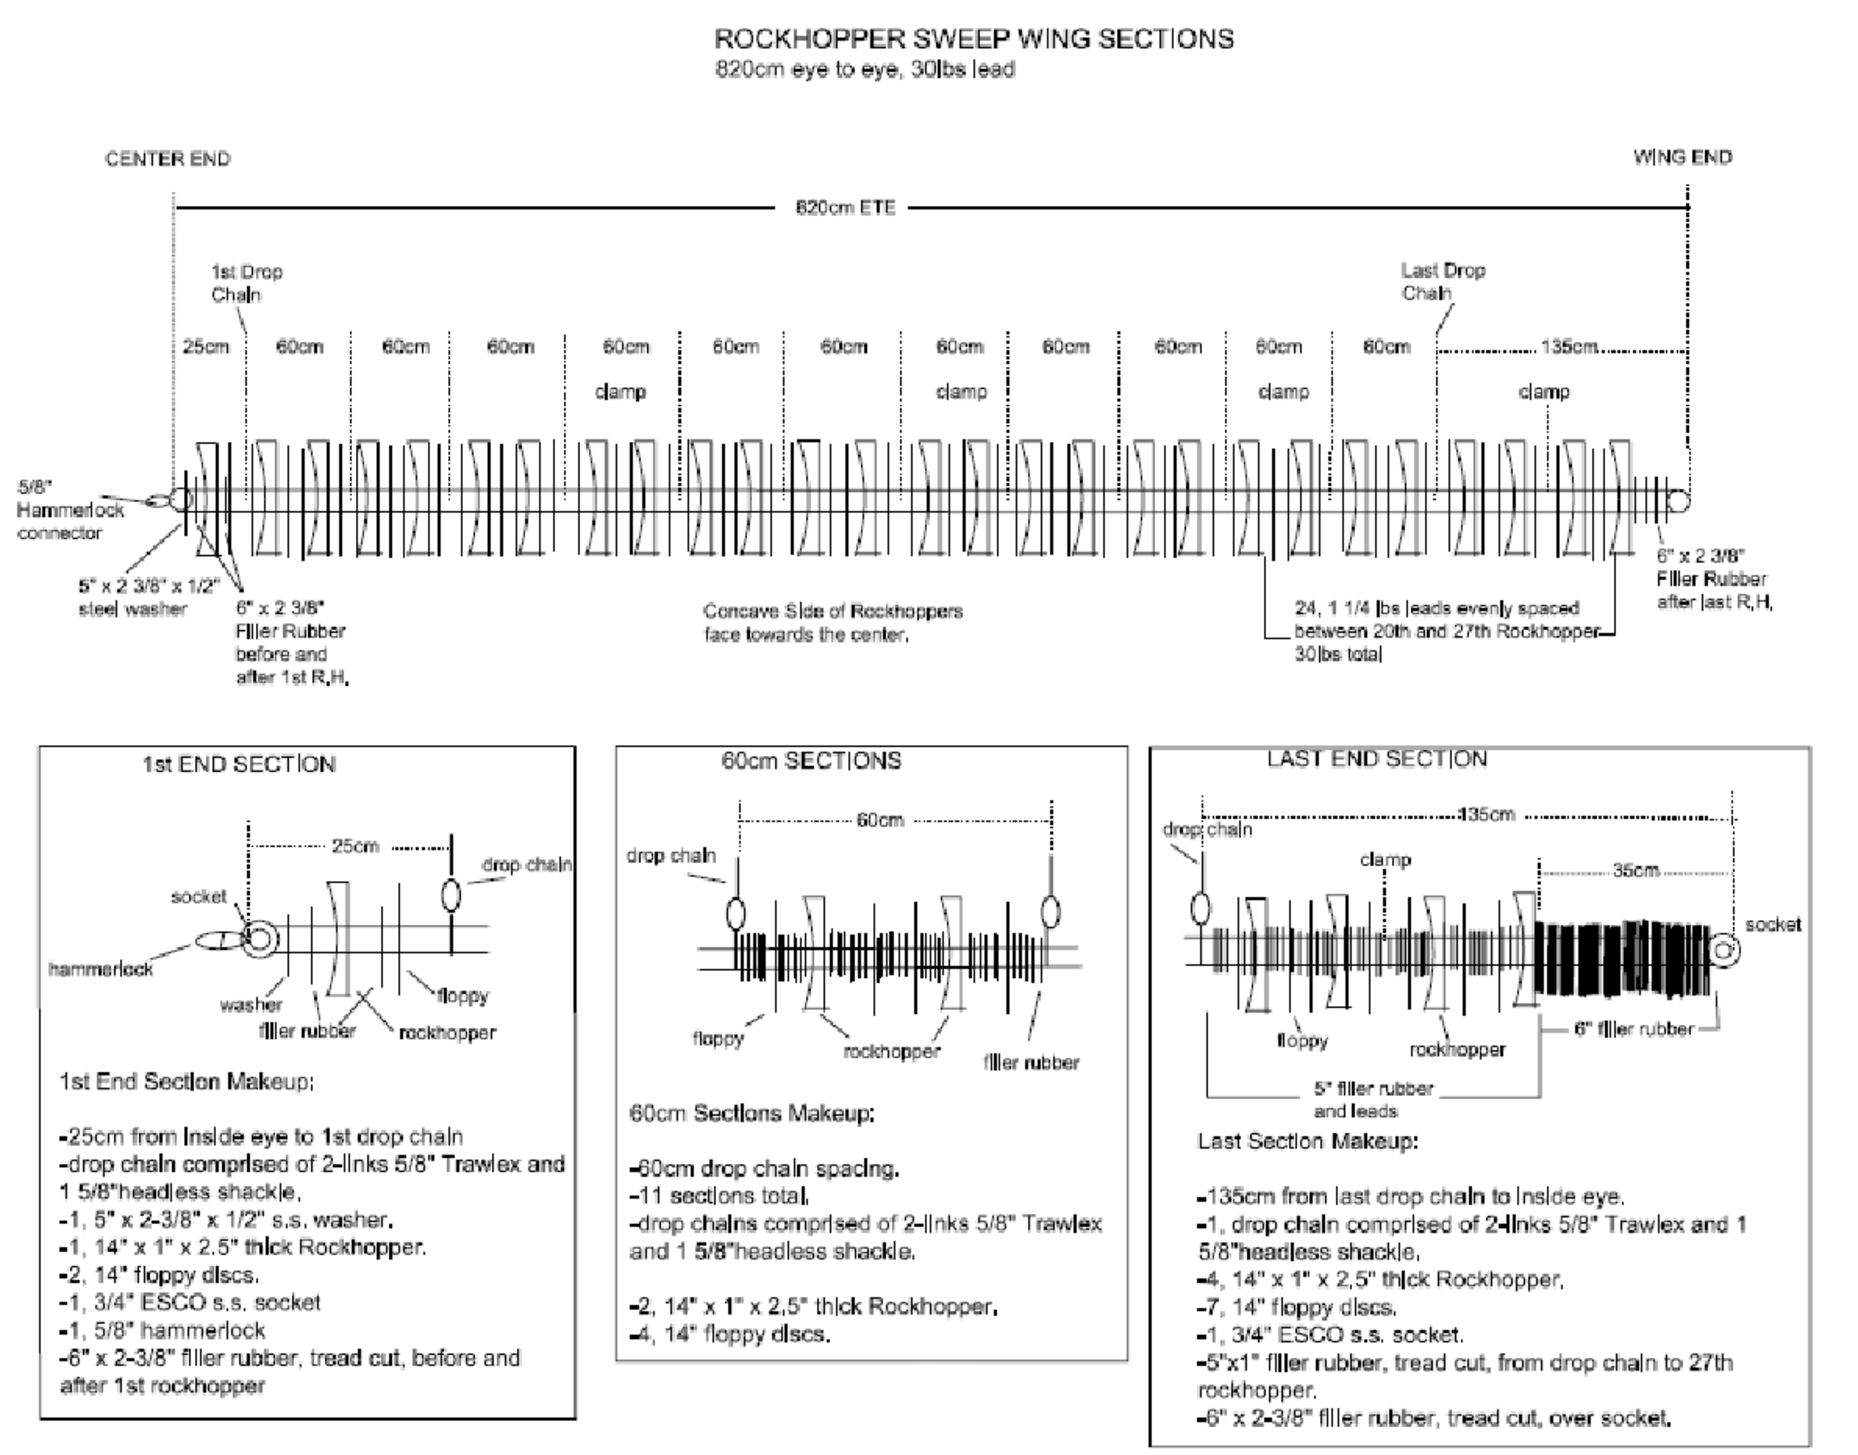
\includegraphics[width = 0.7\textwidth]{rockhopper_schematic_2.pdf}
\end{center}
\end{figure}
\clearpage

\begin{figure}
\caption{Diagram of the chain sweep designed maximize bottom contact and flatfish capture.}\label{chainsweep_schematic}
\begin{center}
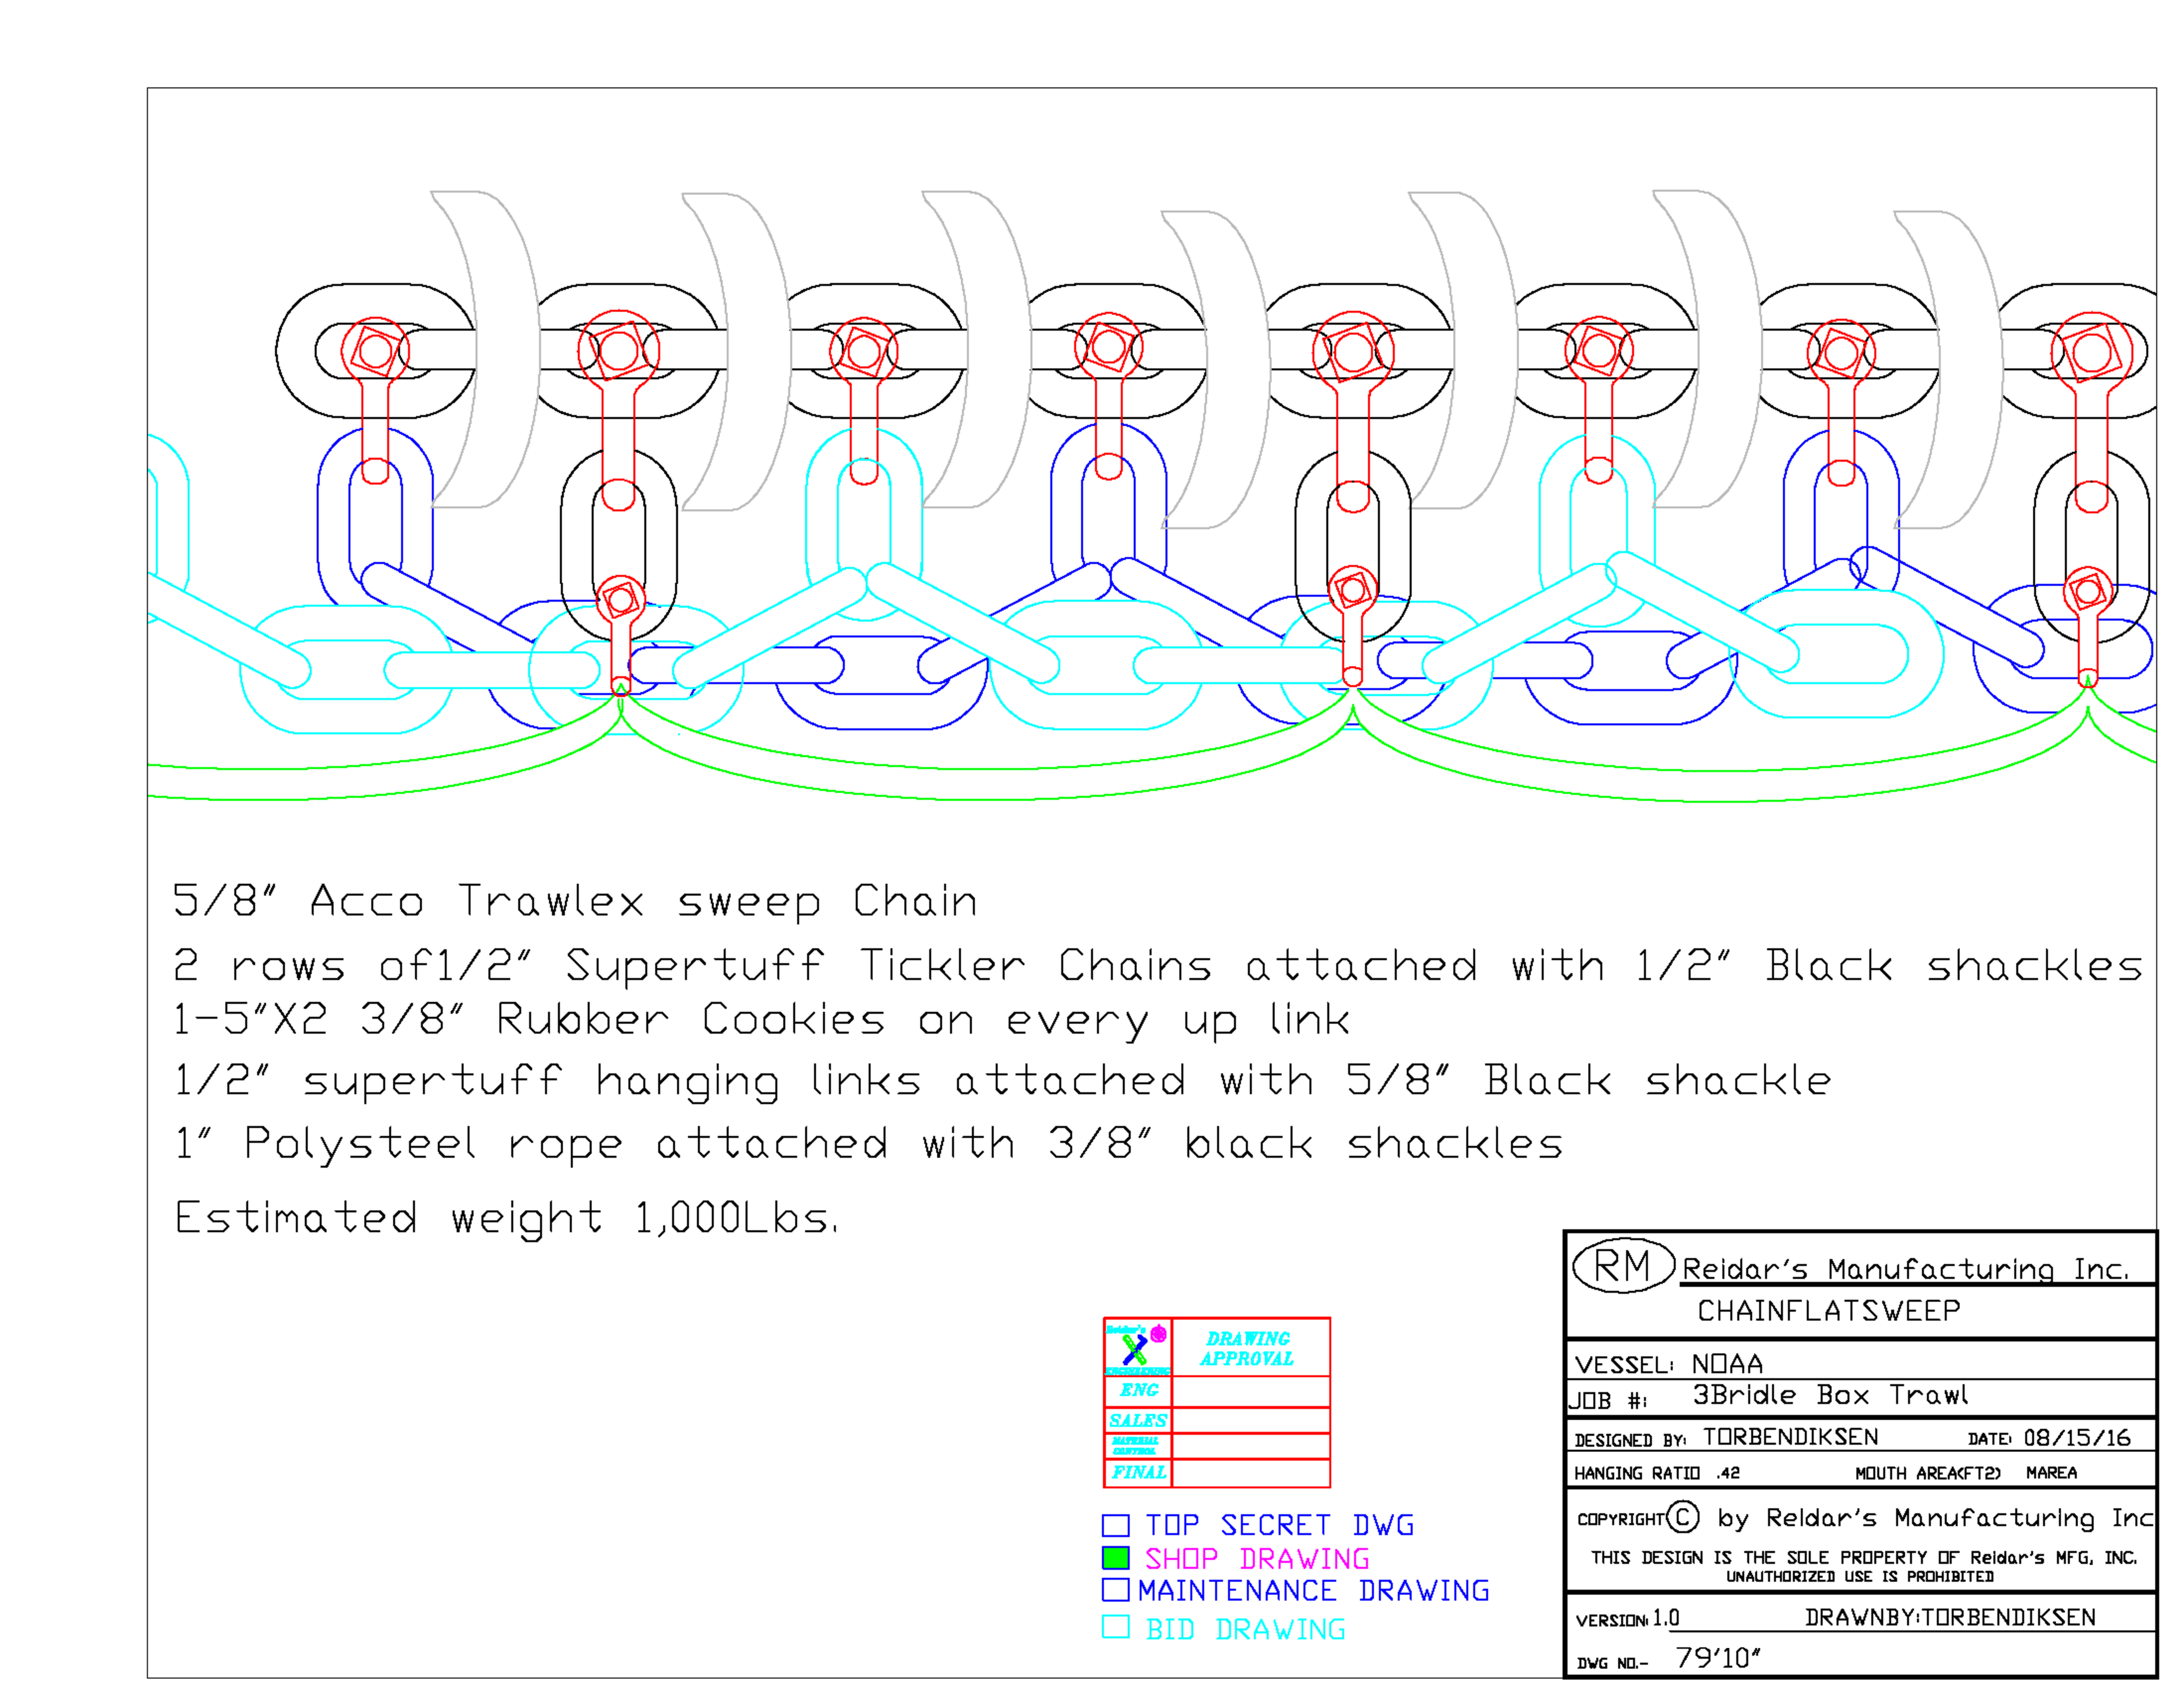
\includegraphics[width = \textwidth]{chainsweep_schematic.pdf}
\end{center}
\end{figure}
\clearpage


\begin{figure}
\caption{Locations of stations in 2017 where the F/V Karen Elizabeth conducted twin-trawl sets with the standard bottom trawl gear and the gear with a chain sweep instead of the rockhopper sweep.}\label{2017_tow_locations}
\begin{center}
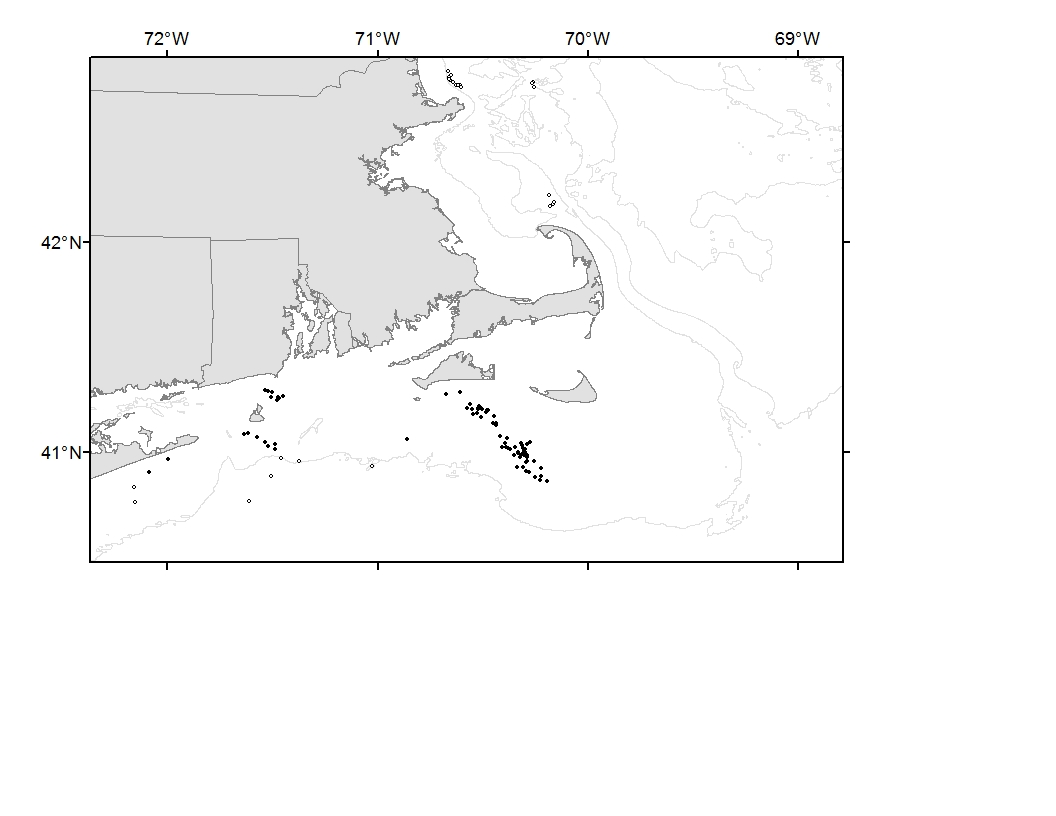
\includegraphics[width = \textwidth]{2017_tow_locations.png}
\end{center}
\end{figure}

\begin{landscape}

\begin{figure}
\caption{Estimated relative catch efficiency of American plaice from the best model (BB$_7$). Black and grey lines are for mean and tow-specific relative catch efficiencies, respectively. Gray polygons and dashed red lines reflect 95\% confidence intervals using derived from delta method-based variance estimates and bootstrap quantiles, respectively.}\label{combined_rhos_plaice}
\begin{center}
\includegraphics[width = 1.5\textwidth]{/home/tmiller2/work/paired_tow_studies/R/2020/plaice/plaice_bb7_rho_1_2.png}
\end{center}
\end{figure}

\begin{figure}
\caption{Estimated relative catch efficiency of winter flounder from the best model (BI$_5$). Black and grey lines are for mean and tow-specific relative catch efficiencies, respectively. Gray polygons and dashed red lines reflect 95\% confidence intervals using derived from delta method-based variance estimates and bootstrap quantiles, respectively.}\label{combined_rhos_winter}
\begin{center}
\includegraphics[width = 1.5\textwidth]{/home/tmiller2/work/paired_tow_studies/R/2020/winter_flounder/winter_flounder_bi5_rho_1_2.png}
\end{center}
\end{figure}

\begin{figure}
\caption{Estimated relative catch efficiency of windowpane flounder from the best model (BI$_6$). Black and grey lines are for mean and tow-specific relative catch efficiencies, respectively. Gray polygons and dashed red lines reflect 95\% confidence intervals using derived from delta method-based variance estimates and bootstrap quantiles, respectively.}\label{combined_rhos_windowpane}
\begin{center}
\includegraphics[width = 1.5\textwidth]{/home/tmiller2/work/paired_tow_studies/R/2020/windowpane/windowpane_bi6_rho_1_2.png}
\end{center}
\end{figure}

\begin{figure}
\caption{Estimated relative catch efficiency of summer flounder from the best model (BI$_5$). Black and grey lines are for mean and tow-specific relative catch efficiencies, respectively. Gray polygons and dashed red lines reflect 95\% confidence intervals using derived from delta method-based variance estimates and bootstrap quantiles, respectively.}\label{combined_rhos_fluke}
\begin{center}
\includegraphics[width = 1.5\textwidth]{/home/tmiller2/work/paired_tow_studies/R/2020/fluke/fluke_bi5_rho_1_2.png}
\end{center}
\end{figure}

\begin{figure}
\caption{Estimated relative catch efficiency of witch flounder from the best model (BB$_8$). Black and grey lines are for mean and tow-specific relative catch efficiencies, respectively. Gray polygons and dashed red lines reflect 95\% confidence intervals using derived from delta method-based variance estimates and bootstrap quantiles, respectively.}\label{combined_rhos_witch}
\begin{center}
\includegraphics[width = 1.5\textwidth]{/home/tmiller2/work/paired_tow_studies/R/2020/witch_flounder/witch_flounder_bb8_rho_1_2.png}
\end{center}
\end{figure}

\begin{figure}
\caption{Estimated relative catch efficiency of yellowtail flounder from the best model (BB$_8$). Black and grey lines are for mean and tow-specific relative catch efficiencies, respectively. Gray polygons and dashed red lines reflect 95\% confidence intervals using derived from delta method-based variance estimates and bootstrap quantiles, respectively.}\label{combined_rhos_ytf}
\begin{center}
\includegraphics[width = 1.5\textwidth]{/home/tmiller2/work/paired_tow_studies/R/2020/yellowtail_flounder/yellowtail_flounder_bb8_rho_1_2.png}
\end{center}
\end{figure}

\begin{figure}
\caption{Estimated relative catch efficiency of red hake from the best model (BB$_9$). Black and grey lines are for mean and tow-specific relative catch efficiencies, respectively. Gray polygons and dashed red lines reflect 95\% confidence intervals using derived from delta method-based variance estimates and bootstrap quantiles, respectively.}\label{combined_rhos_redhake}
\begin{center}
\includegraphics[width = 1.5\textwidth]{/home/tmiller2/work/paired_tow_studies/R/2020/red_hake/red_hake_bb9_rho_1_2.png}
\end{center}
\end{figure}
\end{landscape}

\begin{figure}
\caption{Estimated annual chain sweep-based biomass of American plaice during the fall and spring surveys between 2009 and 2019. Estimates use relative catch efficiency from the best model (BB$_7$). Gray polygons reflect 95\% confidence intervals derived from bootstrap quantiles.}\label{plaice_biomass}
\begin{center}
\includegraphics[width = 0.9\textwidth]{/home/tmiller2/work/paired_tow_studies/R/2020/plaice/plaice_biomass.png}
\end{center}
\end{figure}

\begin{figure}
\caption{Estimated annual chain sweep-based biomass of Georges Bank winter flounder during the fall and spring surveys between 2009 and 2019. Estimates use relative catch efficiency from the best model (BI$_5$). Gray polygons reflect 95\% confidence intervals derived from bootstrap quantiles.}\label{gb_winter_flounder_biomass}
\begin{center}
\includegraphics[width = 0.9\textwidth]{/home/tmiller2/work/paired_tow_studies/R/2020/winter_flounder/gb_winter_flounder_biomass.png}
\end{center}
\end{figure}

\begin{figure}
\caption{Estimated annual chain sweep-based biomass of Gulf of Maine winter flounder during the fall and spring surveys between 2009 and 2019. Estimates use relative catch efficiency from the best model (BI$_5$). Gray polygons reflect 95\% confidence intervals derived from bootstrap quantiles.}\label{gom_winter_flounder_biomass}
\begin{center}
\includegraphics[width = 0.9\textwidth]{/home/tmiller2/work/paired_tow_studies/R/2020/winter_flounder/gom_winter_flounder_biomass.png}
\end{center}
\end{figure}

\begin{figure}
\caption{Estimated annual chain sweep-based biomass of Southern New England winter flounder during the fall and spring surveys between 2009 and 2019. Estimates use relative catch efficiency from the best model (BI$_5$). Gray polygons reflect 95\% confidence intervals derived from bootstrap quantiles.}\label{sne_winter_flounder_biomass}
\begin{center}
\includegraphics[width = 0.9\textwidth]{/home/tmiller2/work/paired_tow_studies/R/2020/winter_flounder/sne_winter_flounder_biomass.png}
\end{center}
\end{figure}

\begin{figure}
\caption{Estimated annual chain sweep-based biomass of Georges Bank-Gulf of Maine windowpane flounder during the fall and spring surveys between 2009 and 2019. Estimates use relative catch efficiency from the best model (BI$_6$). Gray polygons reflect 95\% confidence intervals derived from bootstrap quantiles.}\label{gbgom_windowpane_biomass}
\begin{center}
\includegraphics[width = 0.9\textwidth]{/home/tmiller2/work/paired_tow_studies/R/2020/windowpane/gbgom_windowpane_biomass.png}
\end{center}
\end{figure}

\begin{figure}
\caption{Estimated annual chain sweep-based biomass of Southern New England-Mid-Atlantic Bight windowpane flounder during the fall and spring surveys between 2009 and 2019. Estimates use relative catch efficiency from the best model (BI$_6$). Gray polygons reflect 95\% confidence intervals derived from bootstrap quantiles.}\label{snemab_windowpane_biomass}
\begin{center}
\includegraphics[width = 0.9\textwidth]{/home/tmiller2/work/paired_tow_studies/R/2020/windowpane/snemab_windowpane_biomass.png}
\end{center}
\end{figure}

\begin{figure}
\caption{Estimated annual chain sweep-based biomass of northern red hake during the fall and spring surveys between 2009 and 2019. Estimates use relative catch efficiency from the best model (BB$_9$). Gray polygons reflect 95\% confidence intervals derived from bootstrap quantiles.}\label{north_red_hake_biomass}
\begin{center}
\includegraphics[width = 0.9\textwidth]{/home/tmiller2/work/paired_tow_studies/R/2020/red_hake/north_red_hake_biomass.png}
\end{center}
\end{figure}

\begin{figure}
\caption{Estimated annual chain sweep-based biomass of southern red hake during the fall and spring surveys between 2009 and 2019. Estimates use relative catch efficiency from the best model (BB$_9$). Gray polygons reflect 95\% confidence intervals derived from bootstrap quantiles.}\label{south_red_hake_biomass}
\begin{center}
\includegraphics[width = 0.9\textwidth]{/home/tmiller2/work/paired_tow_studies/R/2020/red_hake/south_red_hake_biomass.png}
\end{center}
\end{figure}



%\begin{table}\caption{Number of twin-trawl tows conducted where each species was caught during the day, night, and in total.}\label{nobs_table}
%\input{nobs_table}
%\end{table}

\begin{landscape}
\begin{table}\caption{Description of relative catch efficiency ($\rho$) and dispersion ($\phi$) parameterizations for conditional binomial and beta-binomial models and corresponding maximized marginal log-likelihood, number of fixed effects parameters ($P$) and $\Delta$AIC for American plaice.}\label{models_table_plaice}
{\Little  \input{../../R/2020/plaice/models_table}}
\end{table}
\end{landscape}

\begin{landscape}
\begin{table}\caption{Description of relative catch efficiency ($\rho$) and dispersion ($\phi$) parameterizations for conditional binomial and beta-binomial models and corresponding maximized marginal log-likelihood, number of fixed effects parameters ($P$) and $\Delta$AIC for winter flounder.}\label{models_table_winter}
{\Little  \input{../../R/2020/winter_flounder/models_table}}
\end{table}
\end{landscape}

\begin{landscape}
\begin{table}\caption{Description of relative catch efficiency ($\rho$) and dispersion ($\phi$) parameterizations for conditional binomial and beta-binomial models and corresponding maximized marginal log-likelihood, number of fixed effects parameters ($P$) and $\Delta$AIC for windowpane flounder.}\label{models_table_windowpane}
{\Little  \input{../../R/2020/windowpane/models_table}}
\end{table}
\end{landscape}

\begin{landscape}
\begin{table}\caption{Description of relative catch efficiency ($\rho$) and dispersion ($\phi$) parameterizations for conditional binomial and beta-binomial models and corresponding maximized marginal log-likelihood, number of fixed effects parameters ($P$) and $\Delta$AIC for summer flounder.}\label{models_table_fluke}
{\Little  \input{../../R/2020/fluke/models_table}}
\end{table}
\end{landscape}

\begin{landscape}
\begin{table}\caption{Description of relative catch efficiency ($\rho$) and dispersion ($\phi$) parameterizations for conditional binomial and beta-binomial models and corresponding maximized marginal log-likelihood, number of fixed effects parameters ($P$) and $\Delta$AIC for witch flounder.}\label{models_table_witch}
{\Little  \input{../../R/2020/witch_flounder/models_table}}
\end{table}
\end{landscape}

\begin{landscape}
\begin{table}\caption{Description of relative catch efficiency ($\rho$) and dispersion ($\phi$) parameterizations for conditional binomial and beta-binomial models and corresponding maximized marginal log-likelihood, number of fixed effects parameters ($P$) and $\Delta$AIC for yellowtail flounder.}\label{models_table_ytf}
{\Little  \input{../../R/2020/yellowtail_flounder/models_table}}
\end{table}
\end{landscape}

\begin{landscape}
\begin{table}\caption{Description of relative catch efficiency ($\rho$) and dispersion ($\phi$) parameterizations for conditional binomial and beta-binomial models and corresponding maximized marginal log-likelihood, number of fixed effects parameters ($P$) and $\Delta$AIC for red hake.}\label{models_table_redhake}
{\Little  \input{../../R/2020/red_hake/models_table}}
\end{table}
\end{landscape}

\begin{table}
\begin{center}
\caption{Estimated chain sweep swept area seasonal survey biomass (mt) for American plaice between 2009 and 2019 using relative efficiency estimates from the best performing model (BB$_7$).}\label{biomass_table_plaice}
{\input{../../R/2020/plaice/biomass_estimates.tex}}
\end{center}
\end{table}

\begin{table}
\begin{center}
\caption{Estimated chain sweep swept area seasonal survey biomass (mt) for winter flounder stocks between 2009 and 2019 using relative efficiency estimates from the best performing model (BI$_5$).}\label{biomass_table_winter}
{\input{../../R/2020/winter_flounder/biomass_estimates.tex}}
\end{center}
\end{table}

\begin{table}
\begin{center}
\caption{Estimated chain sweep swept area seasonal survey biomass (mt) for windowpane flounder stocks between 2009 and 2019 using relative efficiency estimates from the best performing model (BI$_6$).}\label{biomass_table_windowpane}
{\input{../../R/2020/windowpane/biomass_estimates.tex}}
\end{center}
\end{table}

\begin{table}
\begin{center}
\caption{Estimated chain sweep swept area seasonal survey biomass (mt) for summer flounder between 2009 and 2019 using relative efficiency estimates from the best performing model (BI$_5$).}\label{biomass_table_fluke}
{\input{../../R/2020/fluke/biomass_estimates.tex}}
\end{center}
\end{table}

\begin{table}
\begin{center}
\caption{Estimated chain sweep swept area seasonal survey biomass (mt) for witch flounder between 2009 and 2019 using relative efficiency estimates from the best performing model (BB$_8$).}\label{biomass_table_witch}
{\input{../../R/2020/witch_flounder/biomass_estimates.tex}}
\end{center}
\end{table}

\begin{table}
\begin{center}
\caption{Estimated chain sweep swept area seasonal survey biomass (mt) for yellowtail flounder stocks between 2009 and 2019 using relative efficiency estimates from the best performing model (BB$_8$).}\label{biomass_table_ytf}
{\input{../../R/2020/yellowtail_flounder/biomass_estimates.tex}}
\end{center}
\end{table}

\begin{table}
\begin{center}
\caption{Estimated chain sweep swept area seasonal survey biomass (mt) for red hake stocks between 2009 and 2019 using relative efficiency estimates from the best performing model (BB$_8$).}\label{biomass_table_redhake}
{\input{../../R/2020/red_hake/biomass_estimates.tex}}
\end{center}
\end{table}


\begin{table}
\begin{center}
\caption{Implicit annual and seasonal efficiencies of unconverted swept area biomass estimates as measured by the ratio to the chainsweep-based estimates for American plaice in Table \ref{biomass_table_plaice}.}\label{biomass_efficiencies_plaice}
{\input{../../R/2020/plaice/biomass_efficiency.tex}}
\end{center}
\end{table}

\begin{table}
\begin{center}
\caption{Implicit annual and seasonal efficiencies of unconverted swept area biomass estimates as measured by the ratio to the chainsweep-based estimates for winter flounder stocks in Table \ref{biomass_table_winter}.}\label{biomass_efficiencies_winter}
{\input{../../R/2020/winter_flounder/biomass_efficiency.tex}}
\end{center}
\end{table}

\begin{table}
\begin{center}
\caption{Implicit annual and seasonal efficiencies of unconverted swept area biomass estimates as measured by the ratio to the chainsweep-based estimates for windowpane flounder stocks in Table \ref{biomass_table_windowpane}.}\label{biomass_efficiencies_windowpane}
{\input{../../R/2020/windowpane/biomass_efficiency.tex}}
\end{center}
\end{table}

\begin{table}
\begin{center}
\caption{Implicit annual and seasonal efficiencies of unconverted swept area biomass estimates as measured by the ratio to the chainsweep-based estimates for summer flounder in Table \ref{biomass_table_fluke}.}\label{biomass_efficiencies_fluke}
{\input{../../R/2020/fluke/biomass_efficiency.tex}}
\end{center}
\end{table}

\begin{table}
\begin{center}
\caption{Implicit annual and seasonal efficiencies of unconverted swept area biomass estimates as measured by the ratio to the chainsweep-based estimates for witch flounder in Table \ref{biomass_table_witch}.}\label{biomass_efficiencies_witch}
{\input{../../R/2020/witch_flounder/biomass_efficiency.tex}}
\end{center}
\end{table}

\begin{table}
\begin{center}
\caption{Implicit annual and seasonal efficiencies of unconverted swept area biomass estimates as measured by the ratio to the chainsweep-based estimates for yellowtail flounder stocks in Table \ref{biomass_table_ytf}.}\label{biomass_efficiencies_ytf}
{\input{../../R/2020/yellowtail_flounder/biomass_efficiency.tex}}
\end{center}
\end{table}

\begin{table}
\begin{center}
\caption{Implicit annual and seasonal efficiencies of unconverted swept area biomass estimates as measured by the ratio to the chainsweep-based estimates for red hake stocks in Table \ref{biomass_table_redhake}.}\label{biomass_efficiencies_redhake}
{\input{../../R/2020/red_hake/biomass_efficiency.tex}}
\end{center}
\end{table}

%\begin{table}
%\begin{center}
%\caption{Ratios of annual and seasonal unconverted biomass estimates made using numbers at length and estimated weight at length to those %using the aggregate catch (kg) per tow observations.}\label{biomass_ratios}
%{\input{biomass_ratios.tex}}
%\end{center}
%\end{table}

\end{document}
